\documentclass[border=5pt]{standalone}
\usepackage{fontspec,unicode-math}
\setmainfont{Noto Serif}
\setmathfont{STIXTwoMath-Regular.otf}
\usepackage{tikz}
\usetikzlibrary{arrows.meta,calc,patterns,decorations.markings}
\definecolor{Ink}{HTML}{000000}
\tikzset{ax/.style={draw=Ink,line width=.65pt,-{Latex[length=2.2mm,width=1.25mm]}},
lev/.style={draw=Ink,line width=1.25pt,line cap=butt},
fine/.style={draw=Ink,line width=.60pt},
band/.style={draw=Ink,line width=.62pt},
sol/.style={draw=Ink,line width=1.35pt,line cap=round,line join=round},
ray/.style={draw=Ink,line width=.72pt,-{Latex[length=2.0mm,width=1.15mm]}},
dim/.style={draw=Ink,line width=.60pt,{Latex[length=1.7mm,width=.95mm]}-{Latex[length=1.7mm,width=.95mm]}},
lab/.style={text=Ink,font=\fontsize{13}{16}\selectfont,inner sep=1.1pt},
small/.style={text=Ink,font=\fontsize{11}{13}\selectfont,inner sep=1.0pt}}
\pagestyle{empty}
\def\datadir{data}
\IfFileExists{data/F20_1_heat.dat}{}{\def\datadir{../data}}
\begin{document}
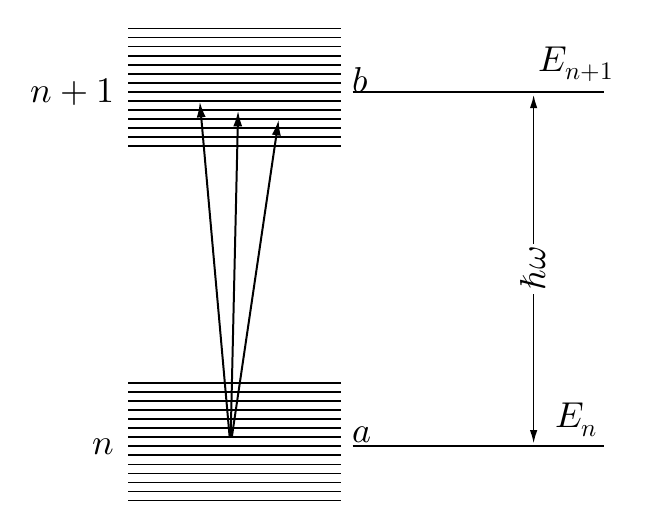
\begin{tikzpicture}[x=1cm,y=1cm]
\def\dy{.115}\def\yb{.65}\def\yt{5.15}
\foreach \i in {0,...,13}{
 \draw[band] (.85,{\yb+\dy*\i})--(3.55,{\yb+\dy*\i});
 \draw[band] (.85,{\yt+\dy*\i})--(3.55,{\yt+\dy*\i});
}
\coordinate (A) at (2.15,{\yb+6*\dy});
\coordinate (B1) at (1.75,{\yt+6*\dy});
\coordinate (B2) at (2.25,{\yt+5*\dy});
\coordinate (B3) at (2.78,{\yt+4*\dy});
% The six sectors keep their own band membership. All three arrows leave A
% and end at distinct actual levels B1,B2,B3, with a small clearance to ink.
\foreach \p in {B1,B2,B3}{\draw[ray,shorten <=3.5pt,shorten >=3.5pt] (A)--(\p);}
\node[lab,anchor=east] at (.72,{\yb+6*\dy}) {$n$};
\node[lab,anchor=east] at (.72,{\yt+6*\dy}) {$n+1$};
\node[lab,anchor=west] at (3.65,{\yb+6*\dy+.15}) {$a$};
\node[lab,anchor=west] at (3.65,{\yt+6*\dy+.15}) {$b$};
\draw[fine] (3.70,{\yb+6*\dy})--(6.9,{\yb+6*\dy});
\draw[fine] (3.70,{\yt+6*\dy})--(6.9,{\yt+6*\dy});
\draw[dim] (6.0,{\yb+6*\dy+.035})--(6.0,{\yt+6*\dy-.035});
\node[lab,rotate=90,fill=white] at (6.0,3.59) {$\hbar\omega$};
\node[lab,anchor=south] at (6.55,{\yb+6*\dy+.08}) {$E_n$};
\node[lab,anchor=south] at (6.55,{\yt+6*\dy+.08}) {$E_{n+1}$};
\end{tikzpicture}
\end{document}
